\documentclass[
  a4paper,            % DIN A4
  DIV=10,             % Schriftgröße und Satzspiegel
  oneside,            % einseitiger Druck
  BCOR=5mm,           % Bindungskorrektur
  parskip=half,       % Halber Abstand zwischen Absätzen
  numbers=noenddot,   % Kein Punkt hinter Kapitelnummern
  bibtotoc,           % Literaturverzeichnis im Inhaltsverzeichnis
  listof=totoc,       % Abbildungs- und Tabellenverzeichnis im Inhaltsverzeichnis
  table
]{scrreprt}
\usepackage{../style/thesisstyle}

\makeglossaries           % create all glossary entries (remember: run makeglossaries manually)
\loadglsentries{thesisglossaries.tex}  % load acronym, symbol and glossary entries

\sisetup{locale = DE}     % siunitx locale setup
%\DeclareSIUnit \fps{fps}  % a custom unit (usage: \SI{24}{\fps})

\begin{document}
% !TEX root = ../thesis.tex
%
% configurations
%

% English Language support
% -> uncomment if needed
% Beta!
%\fullenglish{yes}
\fullenglish{no}

% text field
%-> replace supervisor names with correct ones
\firstSupervisor{Prof. Dr. Philipp Jenke}
\secondSupervisor{Prof. Dr. Peer Stelldinger}

% text field
%-> replace title with your thesis title
\thesisTitle{Beispiel-basierte inverse prozedurale Generierung für zweidimensionale Szenen}
\thesisTitleEN{Example-based inverse procedural generation for two-dimensional scenes}

% text field
%-> replace the key words with your own key words
\keywordsDE{TODO SCHLÜSSELWÖRTER}
\keywordsEN{TODO KEYWORDS}

% text field
%-> replace the text with a description of the thesis
\abstractDE{TODO ZUSAMMENFASSUNG}
\abstractEN{TODO ABSTRACT}

% text field
%-> replace john with your name
\thesisAuthor{Benjamin Schröder}

% text field
%-> enter the submission date
\submissionDate{11. Juli 2024}

% switch - uncomment only one
%-> uncomment NDA or public
%\NDA{yes}
\NDA{no}

% switch - uncomment only one
%-> uncomment old standard cover or cover Corporate Design 2017
\Cover{CD2017}
%\Cover{CD2017NoLogo}
%\Cover{Std2018}
%\Cover{Std2018_green} 			% with green bar

% switch - uncomment only one
%-> uncomment to show list of figures or not
\ListOfFigures{yes}
%\ListOfFigures{no}

% switch - uncomment only one
%-> uncomment to show list of tables or not
\ListOfTables{yes}
%\ListOfTables{no}

% switch - uncomment only one
%-> uncomment to show list of accronyms or not
\ListOfAccronyms{yes}
%\ListOfAccronyms{no}

% switch - uncomment only one
%-> uncomment to show list of symbols or not
\ListOfSymbols{yes}
%\ListOfSymbols{no}

% switch - uncomment only one
%-> uncomment to show list of glossary entries or not
\Glossary{yes}
%\Glossary{no}

% switch - uncomment only one
%-> uncomment the study course you are in
%\studycourse{ITS}
%\studycourse{TI}
\studycourse{AI}
%\studycourse{WI}
%\studycourse{EI}
%\studycourse{REE}
%\studycourse{BMP}		
%\studycourse{BMP-hp}	 % Internship Report in M&P
%\studycourse{BMT}
%\studycourse{BMT-st}    % Study / home assignment in BMT
%\studycourse{BMT-hp}    % Internship Report in BMT
%\studycourse{MI}
%\studycourse{MIK}
%\studycourse{MA}

\def\imgHeight{100pt}
\def\imgWidth{420pt}
    % load all settings

\hyphenation{Ba-che-lor-the-sis Mas-ter-the-sis}

% Cover page here, no page number
\ICoverPage

% PDF Metadata
% !TEX root = ../thesis.tex
%
% PDF Metadata integration
% @author Thomas Lehmann
%

% PDF Metadata
\hypersetup{
pdftitle={\IthesisTitle},
pdfauthor={\IthesisAuthor},
pdfkeywords={\IkeyWordsEN}
}

% Titlepage is page one even if the number is not shown.
\pagenumbering{roman}
% Title page here
% !TEX root = ../thesis.tex
%
% title page
% @author Thomas Lehmann
% Hints for title page and page numbering: https://en.wikipedia.org/wiki/Title_page
%
\title{\IthesisTitle}   % set latex default title to be used by hyperref in pdf
\author{\IthesisAuthor} % set latex default author to be used by hyperref in pdf

\newpage
\thispagestyle{empty}
{\fontfamily{phv}\selectfont
  \hfuzz=20pt       % suppress warnings due to extension onto page margins

  % Author of thesis
  \vspace*{1cm}
  \begin{minipage}[b]{\textwidth}
    \fontsize{14pt}{20pt}
    \selectfont
    \begin{center}
      \IthesisAuthor
    \end{center}
  \end{minipage}

  % Title of thesis
  \vspace{1.5cm}
  \begin{minipage}[b][0cm][t]{\textwidth}
    \fontsize{18pt}{20pt}
    \selectfont
    \begin{center}
      \IthesisTitle
    \end{center}
  \end{minipage}

  % Important information
  \begin{textblock*}{\textwidth}(40mm,210mm)
    \begin{minipage}[b]{\textwidth}
      \hbadness=10001    % suppress underfull warning due to short text
      \fontfamily{cmr}\selectfont
      \fontsize{12pt}{14pt}
      \selectfont
      \ifdefined\ILanguageEN
        \IthesisKindEN ~submitted for examination in \IthesisExaminationEN \\
        in the study course \textit{\IstudyCourseName} \\
        at the \IthesisDepartmentFullEN \\
        at the \IthesisFacultyFullEN \\
        at University of Applied Science Hamburg\\

        Supervisor: \IfirstSv \\
        \ifdefined\IisTermPaper
          % left blank
        \else
          \ifdefined\IisInternshipReport
	  Supervised: \IsecondSv\\
          \else
        Supervisor: \IsecondSv \\
          \fi\fi
        
        Submitted on: \ISubDate \\
      \else
      	\ifdefined\IisInternshipReport
        \IthesisKindDE ~eingereicht im Rahmen des \IthesisExaminationDE \\	
	\else
        \IthesisKindDE ~eingereicht im Rahmen der \IthesisExaminationDE \\
        \fi
	im Studiengang \textit{\IstudyCourseName} \\
        am \IthesisDepartmentFull \\
        der \IthesisFacultyFull \\
        der Hochschule für Angewandte Wissenschaften Hamburg\\

        Betreuender Prüfer: \IfirstSv \\
        \ifdefined\IisTermPaper
          % left blank
        \else
          \ifdefined\IisInternshipReport
        betriebliche Betreuung: \IsecondSv \\							
	  \else
        Zweitgutachter: \IsecondSv \\
        \fi\fi

        Eingereicht am: \ISubDate \\
      \fi
    \end{minipage}
  \end{textblock*}
}


% Abstract page here
% !TEX root = ../thesis.tex
%
% abstract page
% @author Thomas Lehmann
%
\newpage
\thispagestyle{plain}
\clearpage
\hfuzz=12pt       % suppress warnings due to extenstion onto page margins

\textbf{\IthesisAuthor}

\vspace{0.3cm}
\textbf{Thema der Arbeit}

\IthesisTitle

\vspace{0.3cm}
\textbf{Stichworte}

\IkeyWordsDE

\vspace{0.3cm}
\textbf{Kurzzusammenfassung}

\begin{minipage}{\textwidth}
\IabstractDE
\end{minipage}

\vspace{1.0cm}
\textbf{\IthesisAuthor}

\vspace{0.3cm}
\textbf{Title of Thesis}

\IthesisTitleEN

\vspace{0.3cm}
\textbf{Keywords}

\begin{minipage}{\textwidth}
\IkeyWordsEN
\end{minipage}

\vspace{0.3cm}
\textbf{Abstract}

\IabstractEN


% Table of contents here
\tableofcontents

% List of figures here
\IListOfFigures

% List of tables here
\IListOfTables

% List of accronyms here
\IListOfAccronyms

% List of symbols here
\IListOfSymbols

% Uncomment if list of source code is needed (rarely).
%\lstlistoflistings  % requires package listings, needs to uncommenting of usepackage

% path to the chapters folder is set to find the images used there
\graphicspath{ {./chapters/} }

% Chapters
\clearpage
\pagenumbering{arabic}
% @author Benjamin Schröder
%
\chapter{Einleitung}

\section{Motivation}
% In diesem Abschnitt wird erklärt, wieso die prozedurale Generierung überhaupt so ein wichtiges Thema ist.
% Es wird geklärt, wer davon Gebrauch macht, und wieso es für den entsprechenden Anwender Sinn macht. Dazu zählt
% zum Einen das Einsparen von Ressourcen, aber auch das Umsetzen von Spielkonzepten, die durch die hier vorgestellten
% Verfahren erst möglich werden.
Die Erstellung von fiktiven Welten spielt eine große Rolle in vielen Videospielen, Filmen, Virtual Reality Umgebungen
und weiteren Bereichen der Simulation. Hierfür wird eine Vielzahl an verschiedenen Objekten und Strukturen benötigt, um
ein nicht-repetitives und immersives Erlebnis für den Endnutzer zu schaffen. All dies manuell anzufertigen, stellt vor
allem kleinere Indie-Entwicklerstudios vor eine große Herausforderung und kann die Entwicklungszeit signifikant in die
Länge ziehen. Aber auch in größeren Teams mit einer Vielzahl von Designern nimmt die Erstellung von realistischen Welten einen
Großteil der Entwicklungszeit in Anspruch und kann viele Monate dauern. \cite{10_freiknecht} Hier kann an einigen Stellen
nachgeholfen werden, indem man das Erstellen von Inhalten automatisiert. Entsprechende Prozesse lassen sich dem Bereich
der prozeduralen Generierung zuordnen.

Mithilfe von verschiedensten Verfahren können so z.B. einzelne Dungeons oder sogar ganze Welten und darin enthaltene Gebilde
automatisch erzeugt werden. Diese können eine Grundstruktur für ein komplexeres Design bilden, bei dem die Entwickler dann nur noch
kleinere Details per Hand abändern oder hinzufügen müssen. \cite{10_freiknecht} Andererseits existieren auch viele Videospiele,
wie z.B. Minecraft\footnote{\url{https://www.minecraft.net/} [Letzter Zugriff am 01.07.2024]} oder Terraria\footnote{
\url{https://terraria.org/} [Letzter Zugriff am 01.07.2024]}, die auf prozeduraler
Generierung aufbauen, um ihr Spielkonzept umzusetzen. Konkret wird einem neuen Spieler hier eine komplett neue und einzigartige,
aber dennoch logisch zusammenhängende Welt generiert; dies vollautomatisch und ohne zusätzlichen Aufwand für die Entwickler. Jeder
Spieler bekommt so eine einzigartie Erfahrung geboten und kann das Spiel außerdem gewissermaßen unbegrenzt oft durchspielen, ohne
dass es zu repetitiv wird. So etwas wäre ohne Automatisierung gar nicht erst umsetzbar.

\section{Problemstellung}
% Hier wird dann darauf aufmerksam gemacht, dass es bei diesen Verfahren viele Limitationen gibt. Bei vielen Verfahren
% ist es nötig, manuell Regeln für den Algorithmus zu erstellen, sodass dieser überhaupt arbeiten kann. Dies setzt wiederum
% einiges an Kenntnissen voraus und ist somit nicht für jeden zugänglich. Außerdem werden weitere Probleme aufgezeigt.

% Alte Formulierung:
% Es gibt viele bekannte Verfahren, welche solche Ergebnisse unter der Verwendung von u.a. zellulären Automaten, generativen
% Grammatiken oder Constraint-basierten Graphen erzielen können. \cite{5_van_der_linden_et_al} Ein Großteil dieser Verfahren erfordert jedoch
% menschliches Eingreifen in einigen der Teilschritte. So z.B. muss beim Verwenden einer generativen Grammatik meist bereits eine Menge
% an Produktionsregeln durch einen Menschen vorgegeben werden, bevor die automatische Generierung überhaupt beginnen kann. Das Erstellen
% solcher Regeln ist mit viel Arbeit und Trial-and-Error verbunden und kann ohne ein ausgeprägtes Verständnis des angewandten Verfahrens
% sehr schwierig werden. Dadurch kommt es für viele Designer letztendlich doch nicht in Frage. Auch gibt es Szenarien, in denen die Generierung
% von Inhalten durch den Endnutzer beeinflusst werden kann, so z.B. in Spielen, in denen der Spieler dynamisch mit dem Terrain und anderen
% Strukturen interagieren kann. In einem solchen Fall kann der Entwickler keinen direkten Einfluss auf den Generierungsprozess nehmen und alles
% muss voll automatisiert sein. \cite{14_carli_et_al} Hier setzt diese Arbeit an und untersucht Möglichkeiten zur vollständigen Automatisierung
% solcher Verfahren.

Es gibt viele bekannte Verfahren, welche solche Ergebnisse unter der Verwendung von u.a. generativen
Grammatiken oder Constraint-basierten Graphen erzielen können. \cite{5_van_der_linden_et_al} Ein Großteil dieser Verfahren erfordert jedoch
menschliches Eingreifen in einige der Teilschritte, was in einigen Szenarien zu einem Problem werden kann. Hängt die Generierung von
Inhalten eines Produkts z.B. von Entscheidungen des Endnutzers ab (z.B. in Spielen, in denen der Spieler dynamisch mit
dem Terrain und anderen Strukturen interagiert), so kann der Entwickler keinen direkten Einfluss auf den Generierungsprozess
nehmen und alles muss voll automatisiert sein. \cite{14_carli_et_al} Auch in Projekten, in denen dies nicht der Fall ist und der gesamte Inhalt
im Voraus erstellt wird, kann das Voraussetzen von menschlicher Intervenierung als Teil des Prozesses zu einem Problem werden.
Ein Beispiel hierfür wären Verfahren, die eine generative Grammatik nutzen und voraussetzen, dass dafür zunächst eine Menge an Regeln
durch einen Menschen vorgegeben wird, bevor die automatische Generierung überhaupt beginnen kann (z.B. \cite{33_adams}\footnote{
\url{https://citeseerx.ist.psu.edu/document?repid=rep1&type=pdf&doi=25020f8d955aee07b7dd49a3ec23b1f2a8cf1d06} [Letzter Zugriff am 01.07.2024]}).
Das Erstellen solcher Regeln ist mit viel Arbeit verbunden und kann ohne ein ausgeprägtes Verständnis des angewandten Verfahrens sehr
schwierig werden, wodurch der Einsatz eines solchen Verfahrens für viele Designer letztendlich doch nicht in Frage kommen wird. Hier
setzt diese Arbeit an und untersucht Möglichkeiten zur Automatisierung des Erstellens solcher Regeln.

\section{Ziele und Vorgehen}
% Aus den aufgezeigten Problemen ergibt sich nun der Sinn dieser Arbeit. Inverse Verfahren beheben die oben genannten Probleme
% und sollen deswegen genauer untersucht werden. Es werden verschiedene Verfahren analysiert und miteinander verglichen.
% Anschließend wird ein entsprechendes und vielversprechendes Verfahren im Detail untersucht, theoretisch erläutert und
% dann prototypisch implementiert.
Spezifisch soll versucht werden, Muster in Beispielstrukturen zu identifizieren. Aus diesen Mustern sollen dann Regeln zum Zusammensetzen
von Strukturen mit ähnlichen Eigenschaften abgeleitet werden. Gelingt dies, so muss ein Designer lediglich ein einziges Beispielmodell erstellen und
kann damit eine kreative Vision vorgeben. Alle weiteren Schritte zum Ableiten von Variationen dieses Inputs laufen anschließend automatisch ab.
Dies nennen wir \textit{inverse} prozedurale Generierung,
da der Prozess mit einem soweit fertigen Modell beginnt und daraus dann die Regeln ableitet, statt wie in den klassischen Verfahren zuerst mit
der Erstellung der Regeln zu beginnen. Die Erstellung eines Beispielmodells erfordert zwar nach wie vor die Arbeit eines Designers, anschließend
ist aber kein menschliches Eingreifen mehr nötig und das eigentliche Verfahren läuft vollautomatisch ab.

Es gibt bereits verschiedene Verfahren, die einen solchen Ansatz verfolgen. Diese sind u.a. der Gitter-basierte Wave Function
Collapse Algorithmus von Maxim Gumin \cite{45_gumin} oder die nach Symmetrien suchende inverse prozedurale Modellierung von Bokeloh
et al. \cite{3_bokeloh_et_al}.

Im Rahmen dieser Arbeit werden entsprechende Verfahren grob analysiert, deren Probleme aufgezeigt und anschließend ein neuer Ansatz vorgestellt,
welcher die vorhandenen Probleme minimieren soll. Das Endergebnis der Arbeit soll dann sein, dass die Funktionsweise des neuen Konzepts
ausführlich und verständlich dargestellt, und dieses anschließend prototypisch implementiert wird. Wir begrenzen uns dabei auf die Generierung von
Strukturen im zweidimensionalen Raum. Der gleiche Ansatz kann auch auf den dreidimensionalen Raum erweitert werden, um so vielseitiger einsetzbar zu
sein, jedoch reicht die vereinfachte Betrachtung zum Darstellen aller fundamentalen Konzepte.
% @author Benjamin Schröder
%
\chapter{Grundlagen}
In diesem Kapitel werden einige grundlegende Konzepte behandelt, welche zum Verständnis dieser Arbeit beitragen. Zunächst wird
erklärt, was genau unter dem Begriff der prozeduralen Generierung zu verstehen ist, woraufhin einige der fundamentalen Verfahren
vorgestellt werden.

\section{Prozedurale Generierung}
Prozedurale Generierung, oft auch \gls{ac:pcg}, beschreibt eine Menge von Verfahren zum
algorithmischen Erstellen von Inhalten ("Content"). Dabei handelt es sich meist um Verfahren, die automatisch Texturen
oder verschiedene Gebilde im Kontext von Videospielen erzeugen können, so z.B. Landschaften, Flüsse, Straßennetze,
Städte oder Höhlenstrukturen. Auch Musik kann durch solche Verfahren generiert werden, was für diese Arbeit allerdings
weniger relevant ist. \cite{9_togelius_et_al}

TODO:
- Eingehen auf Zufälligkeit \& deterministisches Verhalten (Reproduzierbarkeit durch Seed) -> Quelle 9
- Eingehen auf Unterscheidung zwischen assisted/non-assisted -> Quelle 14

- Auf Begriffe Prozedural, Content, und Generierung einzeln eingehen ?

Diese Definition ist absichtlich etwas allgemeiner gehalten, da das Aufstellen einer spezifischeren Definition nicht
besonders trivial ist. Das Konzept von \gls{ac:pcg} wurde bereits aus vielen veschiedenen Blickwinkeln beleuchtet und ist für verschiedene
Personen von unterschiedlicher Bedeutung. So hat z.B. ein Game Designer eine etwas andere Perspektive als ein Wissenschaftler, der
sich lediglich in der Theorie mit der Thematik beschäftigt. Verschiedene Definitionen unterscheiden sich in Bezug auf
Zufälligkeit, die Bedeutung von "Content", oder darin, ob und in welchem Umfang menschliche Intervenierung eine Rolle in einem
Verfahren spielen darf. Mit diesem Problem haben sich Togelius et al. \cite{9_togelius_et_al} bereits ausführlich befasst, weshalb dies hier
nicht weiter thematisiert werden soll. Für diese Arbeit soll die oben genannte Definition ausreichen.

\section{Verwendung von PCG}
% evtl. weglassen?
Da die Entwicklung von Videospielen aufgrund der großen Anzahl an benötigten Inhalten sehr schnell sehr aufwändig werden
kann, findet \gls{ac:pcg} vor allem in dieser Industrie einen großen Nutzen. Gerade das Erstellen von immersiven Welten erfordert eine Vielzahl
von verschiedensten detaillierten Modellen und kann manuell nur mit sehr großem Arbeitsaufwand umgesetzt werden. Das Automatisieren der
Generierung von Inhalten kann den Entwicklerstudios hier eine bedeutende Menge an Zeit und Kosten sparen, die dann an anderen
Stellen eingesetzt werden können. In vielen Fällen kann sogar Speicherplatz gespart werden, indem die Generierung der Inhalte
zur Laufzeit stattfindet.

\gls{ac:pcg} hat bereits in vielen bekannten Videospielen Verwendung gefunden. Schon im Jahr 1980 wurde %rogue

TODO: Aufzählen von Spielen mit PCG Algorithmen

\section{Perlin Noise}
Ein fundamentales Konzept im Bereich von \gls{ac:pcg} ist das Verwenden von Rauschfunktionen, oder auch \textit{Noise}.
Der wohl bekannteste Vertreter dieses Konzepts ist das 1985 von Ken Perlin entwickelte \cite{16_perlin} und 2002 verbesserte \cite{18_perlin}
\textit{Perlin Noise}, welches seit dessen Veröffentlichung nicht mehr aus der Welt der Computergrafik wegzudenken ist. Mithilfe von
Perlin Noise können eine Reihe von Zufallswerten erzeugt werden. Hierbei sind sich nah beieinander liegende Werte stets sehr ähnlich und es
gibt keine starken Ausschläge, weshalb der entstehende Verlauf sehr organisch wirkt. Aufgrund von dieser Eigenschaft eignet sich Perlin Noise
perfekt zum Erzeugen von natürlichen Strukturen wie z.B. Hügellandschaften oder Inselgruppen. Generell ist der erzeugte Kurvenverlauf vielseitig
einsetzbar und findet somit in vielen verschiedenen Anwendungen einen Nutzen, darunter auch im Bereich der Animation. \cite{17_lagae_et_al}

TODO: Einfügen von Vergleich zwischen Random Noise und Perlin Noise

Neben der vielseitigen Einsetzbarkeit von Perlin Noise gibt es außerdem den Vorteil, dass dieses Verfahren sehr günstig sowohl in Bezug auf
die Berechnungszeit als auch in Bezug auf die Speicherverwendung ist. Einzelne Punkte im Verlauf lassen sich unabhängig voneinander berechnen,
wodurch sich der Berechnungsprozess wunderbar parallelisieren lässt. Dies wird mit der immer weiter voranschreitenden Entwicklung von
Grafikkarten und Prozessoren auch zu einem immer größeren Vorteil. \cite{17_lagae_et_al}

Perlin Noise kann für eine beliebige Anzahl an Dimensionen berechnet werden. Dazu wird der n-dimensionale Raum in eine reguläre gitterartige
Struktur aufgespalten. Die Punkte auf dem Gitter sind dabei all jene, die an ausschließlich ganzzahligen Koordinaten liegen. Im zweidimensionalen
Raum wäre dies also die Menge an Punkten \(\{(x, y) \ \| \ x, y \in \mathbb{N}\}\). Alle anderen Punkte im Raum befinden sich dann jeweils innerhalb
einer der von den Gitterpunkten aufgespannten Zellen.

\begin{figure}[h]
    \centering
    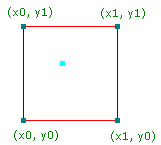
\includegraphics[height=\imgHeight]{images/noise_cell.png}
    \caption{Beispiel einer Gitterzelle im 2D}
    \label{fig:noise_cell}
\end{figure}

Jeder der Gitterpunkte bekommt außerdem einen pseudozufälligen Gradienten (Richtungsvektor der Länge 1) zugeordnet.

\begin{figure}[h]
    \centering
    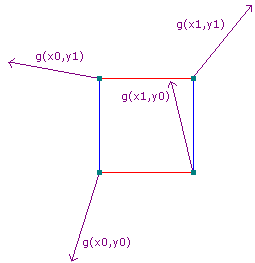
\includegraphics[height=\imgHeight]{images/noise_gradient.png}
    \caption{Pseudozufällige Gradienten für die Eckpunkte einer Zelle im 2D}
    \label{fig:noise_gradient}
\end{figure}

Soll jetzt der Noise-Wert
für einen Punkt im Raum berechnet werden, werden zunächst die Eckpunkte der betroffenen Zelle und deren zugeordnete Gradienten ermittelt.
Außerdem werden die Vektoren berechnet, die von den Eckpunkten in Richtung des aktuellen Punktes zeigen.

\begin{figure}[h]
    \centering
    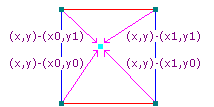
\includegraphics[height=\imgHeight]{images/noise_vectors.png}
    \caption{Vektoren von den Eckpunkten zu einem Punkt im Inneren einer Zelle im 2D}
    \label{fig:noise_vectors}
\end{figure}

Anschließend wird dann für jeden Eckpunkt
das Skalarprodukt aus dem dortigen Gradienten und dem Vektor in Richtung des Punktes gebildet. Der Mittelwert all dieser Skalarprodukte ergibt
dann den finalen Noise-Wert. \cite{16_perlin}\footnote{Erklärung in Anlehnung an https://mzucker.github.io/html/perlin-noise-math-faq.html}

TODO: Erklärung mathematisch beschreiben, Abbildungen erneuern/in eine Abbildung zusammenfassen

\section{L-Systeme}
Ein weiteres bekanntes Konzept ist das der L-Systeme.

\section{Fraktale}
\cite{19_mandelbrot_frame}




example-based model synthesis -> (weitere Merrell Verfahren) -> wave function collapse -> example-based procedural modeling using graph grammars

%\bibliographystyle{plain}
\bibliographystyle{dinat}
\bibliography{literature}

% Appendix
\appendix
% !TEX root = ../thesis.tex
% appendix example chapter
% @author Thomas Lehmann
%

\chapter{Anhang}

\section{Verwendete Hilfsmittel}
In der Tabelle \ref{tab:tooling} sind die im Rahmen der Bearbeitung des Themas der \IthesisKindDE~verwendeten Werkzeuge und Hilfsmittel aufgelistet.

\begin{table}[h!]
\caption{Verwendete Hilfsmittel und Werkzeuge}
\begin{tabular}{|l|l|}
\hline 
\rowcolor{lightgray} Tool & Verwendung \\
\hline
\LaTeX & Textsatz- und Layout-Werkzeug verwendet zur Erstellung dieses Dokuments \\
\hline
 & \\
\hline
\end{tabular}
\label{tab:tooling}
\end{table}



\IGlossary

\Istatement

\end{document}

% compile using the following commands:
%
% pdflatex thesis.tex
% bibtex thesis
% makeglossaries thesis
% pdflatex thesis.tex
% pdflatex thesis.tex
